\section{System architecture}\label{sec:arch}

\subsection{The offline pipeline, stage by stage}\label{sec:arch-pipeline}

The pipeline is a module folder run by path (\texttt{data-pipeline/\allowbreak{}run.py}), not an installed package, and it runs on a
workstation only; continuous integration validates the committed documents and never bakes or trains. Figure~\ref{fig:dataflow}
shows its stages and the documents each writes. The release bake (\texttt{run.py all}) runs, in order: \emph{preprocess}, which
reads \texttt{params.csv} and the survey table and applies the two ingestion contracts; \emph{infer}, which evaluates the
canonical engine at the operating point of each of the $27$ cases; \emph{export}, which writes the trace and the manifest of each
case, measures the lane of the case, checks the expected ranges and the units of every metric, and writes the index; the
\emph{HP500} step, which writes the backbone, the leave-one-survey-out document, the CrusherBayes document and the paired
comparison of the held-out methods; and the readiness
step, which computes the state of every contract from the catalog and the repository. A failing expected range or a value outside
its unit's range stops the bake. The model step (\texttt{run.py models}) is separate because it needs torch: it draws the two
Latin-hypercube sweeps, labels them with the engine, trains the surrogate and the autoencoder, exports them to ONNX, quantises the
surrogate to int8, evaluates both through onnxruntime on the held-out draw, and refreshes the index and readiness. The bake never
trains; it reads the released model bundles as they stand. Every random draw comes from one seeded generator factory, so a run is
a pure function of its inputs and seeds: a full re-bake of release \docrelease{} into a sandbox output root reproduces every committed trace
and the backbone, leave-one-survey-out and CrusherBayes documents byte for byte (Section~\ref{sec:repro}); the comparison
document is a pure function of the last two, and its producer test rebuilds it from them byte for byte.

\begin{figure}[!t]
\centering
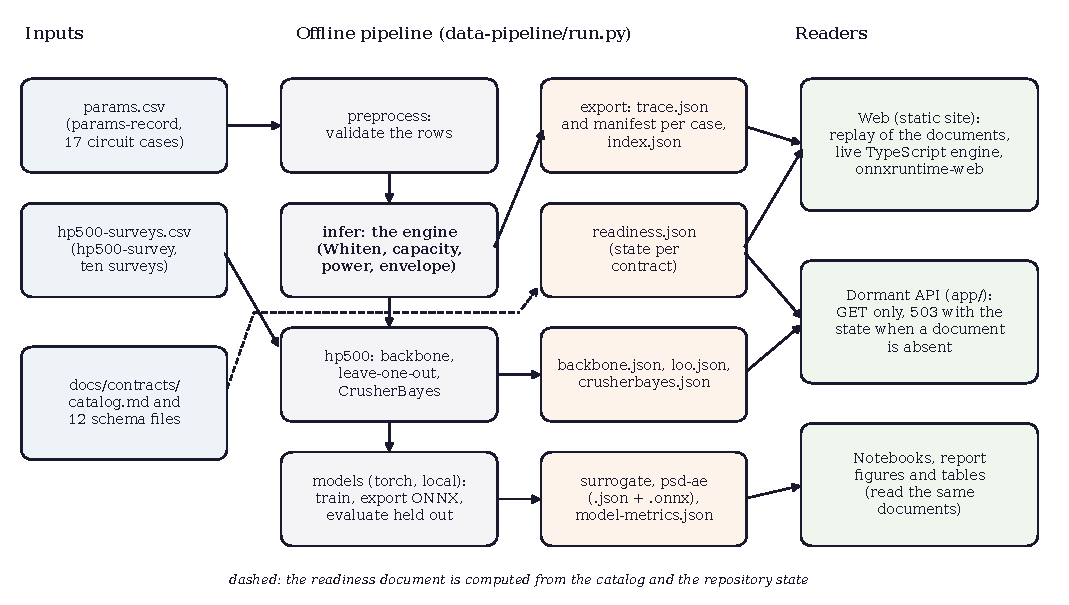
\includegraphics[width=\textwidth]{fig-dataflow.pdf}
\caption{Data flow of the product: the two source tables and the contract catalog enter the offline pipeline, whose stages write
the case traces, manifests and index, the four HP500 documents, the model bundles and their metrics, and the readiness document,
which the static web, the dormant interface and the notebooks read.}
\label{fig:dataflow}
\end{figure}

\subsection{The engine in two languages}\label{sec:arch-engine}

The engine is one vertical implementation written twice. The Python package \texttt{data-pipeline/\allowbreak{}pipeline/\allowbreak{}model/\allowbreak{}crusher/\allowbreak{}} is
canonical: it labels the cases, the sweeps and the surveys. The TypeScript port \texttt{frontend/\allowbreak{}src/\allowbreak{}engine/\allowbreak{}} re-runs a case in the
browser whenever the reader moves one of the six controls. Both are plain arithmetic on IEEE doubles. The Python engine
deliberately avoids library linear algebra: the LU solve with partial pivoting is ported line for line, so the order of the
floating-point operations is the TypeScript order, and a small module reproduces the JavaScript semantics where Python differs (a
negative base with a fractional exponent is not a number, an exponent overflow is infinity, a division by zero is a signed
infinity), so that an out-of-domain point returns a flagged result in both languages instead of raising. A shared reference file
of $\nrefpoints$ operating points holds the two engines equal: every result field and every feature vector agrees within $10^{-9}$
relative, and the largest relative difference measured over the file is $\refworst$. A second test re-runs every baked
case in TypeScript and compares it with its trace to the six significant digits the trace is written with.

The lane of a case is decided by measurement. A case may be re-run live in the browser only when its engine is pure Python with
dependencies inside an allowed set (\texttt{numpy}), when one run completes within $1500$~ms and when its trace is at most
$256$~KiB; otherwise the web would replay the committed artifact. The canonical engine evaluates a case in a median of $\resEngineMed$~ms
(the median over the $27$ cases of the median of seven runs after a warm-up; at most $\resEngineMax$~ms), and the largest trace is $4{,}127$~bytes,
so every case is live-eligible. The measured decision and the two budgets are written into each manifest; the raw run time is not,
because a manifest must not change between two bakes of the same inputs.

\subsection{The web, the learned models in the browser, and the interface}\label{sec:arch-web}

The site is static and is deployed to GitHub Pages; it holds no secret and calls no server. A copy step places exactly the files the
index declares into the site, and the web's types are generated from the contract schemas. The App is a workbench on the shared
CAOS application shell: a case selector, the six controls, and five groups of views with a context tab: System (the circuit, then the
chamber as a two-dimensional section beside a three-dimensional kinematic view of its geometry and motion, which is not a particle
simulation), Product (the size distribution with the classification curve, then the population balance), Performance ($P_{80}$
against operating hours first, then the hours to a target against the drift rate of Figure~\ref{fig:drift}, the result, the setting
and power responses and the variants), Learned (the two learned models) and Validation (the methods compared on the
surveys first). Each group opens on one view of the catalog of Section~\ref{sec:arch-showcase}, and each view draws the live engine
and, dashed, the replay of the committed trace. The two ONNX graphs run in
the browser through onnxruntime-web $1.27.0$, the same release as the Python onnxruntime that evaluates them, as single-threaded
WebAssembly served by the site itself, because a static host does not send the headers that threaded WebAssembly needs. Calls to one
model are serialised, because the runtime forbids concurrent runs on one inference instance. The web encodes the inputs and decodes the outputs
entirely from the model contracts, so a retrained model ships by replacing its contract and its graph.

Every view shows the readiness of the contracts it reads, and every learned answer is labelled with the model that answered: the
surrogate or, when the bundle is invalid or the point is outside the training ranges or on the calibrated lane, the engine. The
dormant interface of \texttt{app/\allowbreak{}} is a FastAPI application with six read-only routes over the committed documents; it is run by its
contract tests and is not deployed.

\subsection{The App's views and the guided story}\label{sec:arch-showcase}

The App is built around a catalog of six views, each of which answers one question of the crushing problem from one or more
contracts of Section~\ref{sec:data}, and a guided story of five steps that walks a reader through them on the real surveys
(Table~\ref{tab:views}). The catalog is fixed in the design document of the product, which names for each view its question, the
contracts it reads, its kind of drawing, its interactions, the views it is linked to and where it is placed; the App and the story
are built on the shared application shell \texttt{@fasl-work/\allowbreak{}caos-app-shell} $0.25.0$ over the product template
\texttt{CAOS\_PRODUCT\_TEMPLATE} $0.15.005$, both pinned to the exact release, so that the workbench, the charts, the anchored callouts,
the linked-view store, the story frame and the measured layout checks come from the shell and are not re-implemented by the product.
Every number a view or a story step shows is read from the committed artifacts or computed by the live engine from them.

\begin{table}[!t]
\centering
\caption{The six views of the App's catalog: what each draws, the question it answers, the contracts it reads, where the App places it
and the step of the guided story that opens on it. Transcribed from the visualization catalog of the product's design document.}
\label{tab:views}
\scriptsize
\begin{tabular}{@{}p{0.12\textwidth} p{0.26\textwidth} p{0.22\textwidth} p{0.17\textwidth} p{0.11\textwidth}@{}}
\toprule
View & What it draws & Question & Contracts & App group; story step \\
\midrule
Circuit & The three-stage crushing circuit as a flowsheet, each stage named by its machine, the selected case's streams labelled
(t/h, $F_{80}$, $P_{80}$, kW, setting), the flow moving at a speed proportional to the throughput & Where does the crusher sit in the
circuit, and what enters and leaves it? & \texttt{case-index}, \texttt{case-manifest}, \texttt{trace} & System, first; Measure \\
Chamber & The three-dimensional cutaway (mantle, concave, gap, feed) beside the two-dimensional section with the nip angle drawn as a
wedge against the grip limit $2\arctan0.35=38.58^\circ$ & How does the chamber's geometry set the product? & \texttt{case-manifest}, the
live engine's chamber & System, second; Look inside \\
Size distribution & Cumulative passing of feed and product on a logarithmic size axis, $F_{80}$ and $P_{80}$ marked, the classification
curve on the same axis & What size distribution does the crusher make, and where do $F_{80}$ and $P_{80}$ sit? & \texttt{trace},
\texttt{case-manifest} & Product, first; Solve \\
Drift & $P_{80}$ against operating hours at the reader's drift rate (against the opening of the setting until one is entered), the target
crossed, the drift response, the $45$~h re-set line & How does the product drift as the liners wear, and when does $P_{80}$ leave its
target? & \texttt{trace}, the live engine's drift functions & Performance, first; Operate \\
Population balance & The Neumann series of the Whiten solve, pass by pass on the size-distribution axes against the closed form, with
the residual and the mass sent back & How does the population balance compute the product? & \texttt{trace}, the live engine's $\mathrm B$,
$C$ and $\mathbf f$ & Product, second; Solve \\
Methods compared & The held-out MAPE of every method per target with the ten per-survey errors, the bands, the recommended method marked
and the paired gap of the selected method as a bracket & Which method should a forecast trust, measured on surveys it never saw? &
\texttt{hp500-loo}, \texttt{hp500-crusherbayes}, \texttt{hp500-comparison}, \texttt{hp500-backbone} & Validation, first; Compare \\
\bottomrule
\end{tabular}
\end{table}

\emph{The six views.} The circuit view answers where the selected crusher sits: a real survey shows its measured feed rate, $F_{80}$,
power and setting from its manifest and the product $P_{80}$ from its trace, a synthetic case its trace and manifest, and a stage with
no case of its machine is refused rather than drawn empty; the flow is a style animation of the drawing with no animation loop of its
own and stands still for a reader who asks for reduced motion. The chamber view draws the geometry the capacity and the nip angle of
Section~\ref{sec:m-capacity} come from: the nip angle between mantle and concave at the engine's value, and the grip limit as a second,
dashed wedge, so that a reader sees how close the chamber is to slipping; the four parts of the three-dimensional cutaway are named on
the canvas and selectable, and the drawing says that it is kinematic and not a particle simulation. The size-distribution view is the
domain's diagram of Section~\ref{sec:m-feed}. The population-balance view shows Equation~\eqref{eq:whiten} at work: the product after
$n$ passes, $\mathbf p_n=(\mathrm I-\mathrm C)\sum_{k<n}(\mathrm B\mathrm C)^k\mathbf f$, converges onto the closed form, and because
$\mathrm B$ is strictly lower triangular the series is exact after at most as many passes as size classes; its tests require the
series at the last pass to equal the engine's product to $10^{-9}$ on cases of every machine. The drift view is the projection of
Section~\ref{sec:m-drift} with the drift response of Section~\ref{sec:results-drift} and the state of the margin to the target by its
meaning. The comparison view reads Section~\ref{sec:results-paired}: it opens on the runner-up, so the recommended and the selected
method differ, draws the paired gap of the selected method as its mean and its $95\%$ interval, and its takeaway says how sure the
ranking is with ten surveys; with the comparison document absent, the gap and that sentence give the readiness reason.

\emph{The guided story.} Five routes, \texttt{/story/\allowbreak{}measure}, \texttt{/story/\allowbreak{}inside}, \texttt{/story/\allowbreak{}solve},
\texttt{/story/\allowbreak{}compare} and \texttt{/story/\allowbreak{}operate}, take a reader through the views in the order of the problem: what was measured (the circuit view on a survey, with
the ten surveys' feed rates drawn on the stage, $813$ to $1639$~t/h), what happens inside the chamber (the section), how the engine
computes the product (the population balance on the size-distribution axes, playing its passes up to the first pass at which the
residual falls below $10^{-6}$), which method to trust (the comparison, whose headline names the setting-only line at its held-out power MAPE of $\cmpPLineMape\%$,
shown to one decimal) and what to do with it (the drift view, whose headline states that $P_{80}$ reaches the
$\drTargetHead$~mm target after $\drOpenHead$~mm of setting drift on survey 1). Each step has a headline that states a number read
from the artifacts or computed by the live engine, a stage with three anchored callouts that carry a value, a unit and a source, and a
docked panel; a unit test asserts every headline's number against its source document or the engine. The exit of each step opens the
App on the step's case and view and, from the last step, on the story's target, so a reader continues where the story stopped.

\emph{Linked selection.} The views share the shell's linked-view store, both ways: a size class selected in the size distribution is
selected in the population balance, a survey selected in the comparison is the case of the circuit and the size distribution, a part
selected in the three-dimensional chamber is selected in the section and its callout, and the pass count of the population balance is
one cursor for both views that draw it. The hours cursor of the drift view is a second instance of the same store, which sets the
setting drawn in the chamber and the product drawn in the size distribution.

\emph{Staged motion and its reduced-motion path.} A change of story step is staged on the shell's staged-transition and camera
functions: the subject changes first (the population balance plays its passes, the comparison grows its methods' dots one by one, the
drift view draws its curve out to the crossing, and the circuit and the chamber move their drawing in), then the subject is
highlighted, the three callouts enter one at a time and the panel builds with its numbers counting. A stage that is still entering
declares the shell's loading state, so the layout checks measure the settled stage. Under the reduced-motion preference every stage
applies at once and its first frame is its final one. Each callout's leader ends on the data point it names: the anchor is placed on
the scales the chart has rendered and is measured again after every render, and a browser check requires every leader to end within
$4$ pixels of its point at phone and desk widths, with and without reduced motion, and measures a leader planted $16$ pixels off as
a miss. The App keeps its primary drawing on at least $60\%$ of the screen, and a story step, measured as its stage and docked panel
together, on at least $80\%$, which the shell's layout check measures.

\subsection{Resources}\label{sec:arch-resources}

Table~\ref{tab:resources} gives what each stage of the pipeline needs on the development workstation (Windows 11, Python
$\resPython$ in the pipeline environment, Node $24$, a processor with $\resThreads$ threads), measured on $\resDate$ with a
process-tree monitor that polls the peak memory of the command and of every process it starts every $20$~ms. The three pipeline
stages that write artifacts (the bake, the HP500 step and the training) were run into a sandbox output root, so the committed artifacts were not rewritten; the disk column of a
sandbox run is the bytes it wrote there, without the released model bundles that the committed tree also holds. No stage needs a
graphics processor or a network after the installation. The bake takes about $\resBakeMin$~minutes, of which the HP500 step takes about
$\resHpMin$: the CrusherBayes sampler fixes the work at $20\times7000=140{,}000$ log-probability evaluations per posterior, each of which
evaluates the engine on the nine or ten training surveys of its fold, for eleven posteriors, which the step spreads over the processor's
threads. Every other stage takes seconds to minutes. The built site is $\resSite$~MB, of which $\resWasm$~MB is the ONNX Runtime WebAssembly binary.

\begin{table}[!t]
\centering
\caption{Measured resources of each stage of the pipeline and the web on the development workstation, measured on $\resDate$: peak
memory of the process tree, disk written and wall time. Generated from \texttt{data/\allowbreak{}resources.json} of the report, which records
each measurement with its exit status.}
\label{tab:resources}
\footnotesize
% generated by figures/make_tables.py; do not edit by hand
\begin{tabular}{@{}p{0.47\textwidth} r r r l@{}}
\toprule
Stage & Peak memory & Disk & Time & Where it runs \\
\midrule
Bake (\texttt{run.py all}: 27 cases, the three HP500 documents, index, readiness) & 1460 MB & 241 KB & 69.5 min & workstation \\
HP500 step alone (\texttt{run.py hp500}: backbone, CrusherCal, the CrusherBayes sampler) & 1456 MB & 28 KB & 58.4 min & workstation \\
Training (\texttt{run.py models}: sweeps, two networks, export, evaluation) & 462 MB & 59 KB & 108.4 s & workstation, CPU \\
Python tests, the whole suite (while other jobs used the workstation; exit status 1: the run had failing tests and is a time measurement only) & 306 MB & none & 29.1 min & workstation \\
Web install (\texttt{npm ci}) & 641 MB & 328.0 MB & 32.4 s & workstation, CI \\
Web build (\texttt{npm run build}) & 618 MB & 17.1 MB & 8.1 s & workstation, CI \\
Web unit tests (409 tests) & 2651 MB & none & 6.8 s & workstation, CI \\
\bottomrule
\end{tabular}

\end{table}
